\chapter{Theoretical Foundation}
\label{chap:theory}

The following chapter provides a theoretical foundation for the research conducted in this thesis. It introduces the basic concepts of material flow planning and simulation, digital twins, process mining, and verification, validation, and uncertainty quantification (VVUQ). The relevance of these concepts in the context of simulation-based digital twins and their application in corporate practice will also be discussed.


\section{Discrete Material Flow Systems and Simulation}
This section begins with an introduction of the underlying concepts of Discrete Material Flow Systems (DMFS) and Simulation Based Digital Twins (SBDT).
\label{sec:material-flow}
\subsection{Basic Concepts}
Discrete material flow systems cannot be fully understood without first clarifying the principles of Discrete Event Simulation (DES) for Discrete Event Systems. In DES, a system changes its state through \textit{events} that occur at specific, discrete time instances; it is assumed that no changes occur between two successive events. Consequently, the state of the system is completely defined by the values of its descriptive variables at each event occurrence \parencite{varga2001discrete}. The time at which an event occurs is typically marked by a timestamp, and the scientific observation of such systems is conducted by analyzing the discrete \textit{sequence} of events over time \parencite{robinson2014simulation}.

Simulation, in this context, refers to the process of imitating the operation of a Discrete Event System over time—often through multiple event sequences. This imitation is captured in a model, and the core activities in a simulation involve constructing and experimenting with this model. A high-quality simulation abstracts the essential features of the system, which requires the modeller to have a sound a priori understanding of what “essential” means in the given context. Although the model can later be refined, its quality is primarily measured by its ability to predict outcomes and offer a diverse range of scenarios \parencite{maria1997introduction}.

In the context of DMFS, their simulation describes the imitation of material flow systems by breaking down continuous flows into discrete events. Such material flow systems can be characterized as “systems processing discrete objects (parts) that move at regular or irregular intervals along transportation routes or conveyor lines, comprising production and logistic systems” \parencite{Arnold2006,schwede2024learning}. These systems form the backbone of material flow planning and control structures. The central idea of material flow planning and control is to ensure that material requirements—both in terms of quantity and timing—are met during transportation and storage across the various stages of the supply chain \autocite{Gehr2007}. Importantly, the time horizon of interest spans from order placement up to delivery.
To summarize, DMFS are often simulated using DES, which abstracts the continuous flow of materials into discrete events. The simulation is carried out using a model. The simulation and modeller are embedded in the context of material flow planning and control, which aims to ensure that material requirements are met across the supply chain. Successfully performed material flow planning and control induce high quality data for simulation and modelling purposes.

\subsection{Comparing DMFS}
Because the simulation of DMFS often involves (discrete) event simulation, events in DMFS need to be further differentiated to be comparable. \Autocite{Arnold2006} propose to differentiate DMFS into static and dynamic components.

Static components describe the possible states of the system. Possible states can be the set of possible processes given a part or resource, for example. Dynamic components define the concrete material flow for a certain part or order.
Static components include parts, resources and processes \autocite{schwede2024learning}. Parts are transformed by processes using resources sometimes based on orders. Transformation can have an impact on physical properties of the parts (transformation model), spatial position (transition model), the quality of the parts (quality model) and takes time (time model) and uses resources (resource model). Resources have a capacity of handling parts in parallel (resource capacity model) and processes have a predecessor-successors relationship (process model).
Dynamic components are used to define the concrete dynamic material flow within the DMFS. There are four components: Order generation, order control, resource control and supply control. Order generation defines the load the system must process. Order control defines how parts are processed, sometimes referred to as routing rules \autocite{mildeautomated}. Resource control defines how resources decide to handle processing requests, also sometimes referred to as priority rules. Supply control describes how supply parts are provided \autocite{mildeautomated,schwede2024learning}. See the latter source for a more detailed description of the components.


\subsection{Production Planning and Control}
Successful companies use production planning and control frameworks to describe and optimize their DMFS. After establishing a theoretical foundation and simulation approaches for DMFS, this section thus focusses on Production Planning and Control (PPC) as a critical factor influencing the quality and quantity of data generated by Discrete Event Simulation.
PPC is the structured approach to planning, scheduling, controlling and managing all aspects of the manufacturing process. It involves the coordination of resources, processes, and orders to meet production goals. PPC is essential for optimizing production processes, reducing costs, and improving quality. The main functions of PPC include production planning, production scheduling, and production control. Production planning involves determining the production capacity, production goals, and production processes. Production scheduling involves creating a detailed schedule for production activities. Production control involves monitoring and controlling production activities to ensure that production goals are met \parencite{kiran2019production}. Scheduling is usually the last step performed before execution of the plan \parencite{pinedo2012design}.

The integration of PPC with simulation models is crucial because it directly affects the data quality used in DES of DMFS. Effective PPC processes anticipate anomalies in the production cycle, allowing for adjustments that maintain system efficiency and reliability. If successful, these adjustments yield high-quality data that enhance the accuracy of simulation outcomes. \parencite{kiran2019production}.


\subsection{Relevant KPIs and Metrics}
Up to this point, DES for SBDT of DMFS has been introduced, outlining the key factors that contribute to a robust simulation. A model differentiation framework proposed by \citeauthor*{schwede2024learning} has been briefly presented to facilitate comparison of SBDT. Furthermore, the critical role of PPC in generating high-quality data for simulation has been discussed. These discussions ignored up till now that, even when SBDT are integrated within well-functioning PPC processes, various SBDT models remain prone to errors and inherent trade-offs that must be addressed by the modeller \parencite{Tao2018ijamt}.

The goal conflict of the modeller when developing SBDT can be described by the following conflict triangle \parencite{robinson2014simulation,balci2012life}:

\begin{figure}[htbp]
  \centering
  
\includegraphics[width=0.8\textwidth]{figures/goals.png}
  \caption{The goal conflict of the modeller when developing SBDT. Aiming for higher accuracy (validity) often leads to higher computational costs (efficiency) and reduced scalability (applicability). Reaching more efficiency often leads to reduced accuracy and scalability. Aiming for higher scalability often leads to reduced accuracy and efficiency.}
  \label{fig:goals}
\end{figure}

Focusing one of the three dimensions—accuracy (validity), efficiency (computation time), and applicability (scalability)—often leads to trade-offs in the other two dimensions. Oftentimes the data itself is not sufficient to make a decision on which trade-off to make. Limited data points may hinder the modeller from reaching high validity. System architecture may block the system from reaching good scalability. Hardware limitations may hinder the modeller from reaching high efficiency.
At other times, corporate management may have a preference for one of the dimensions.

One solution to balance and quantify these goals can be achieved by defining a set of KPIs. Some may already be available through PPC, some may be calculated from DES data or the DES itself. Optimally, the data warehouse provides relevant views \parencite{cui2020manufacturing}. Because the SBDT in theory mirrors the DMFS, the KPIs gathered from PPC and the DES should yield identical values. Deviations between the KPIs of the SBDT and the DMFS may indicate errors in the SBDT or anomalies in the DFMS. The following KPIs are relevant for the evaluation of SBDT:

\begin{figure}[htbp]
  \centering
  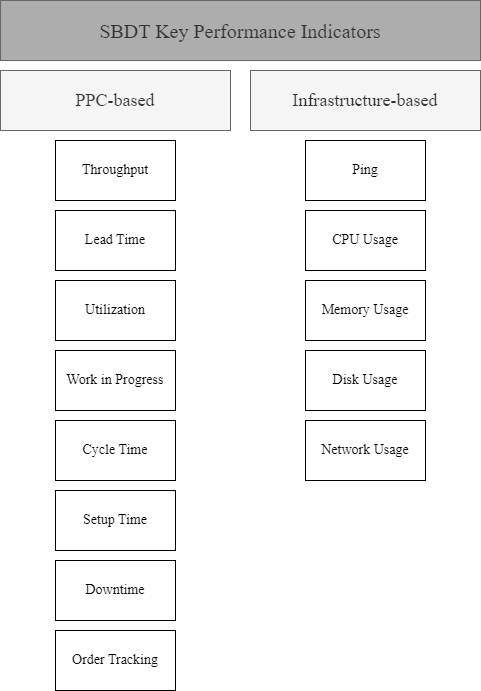
\includegraphics[width=0.8\textwidth]{figures/kpi.png}
  \caption{SBDT KPIs differentiated by PPC-based and Infrastructure-based indicators.}
  \label{fig:kpis}
\end{figure}

The PPC related KPIs may be provided by above mentioned data warehouse, because they are highly relevant in the context of production scheduling and -control. Throughput measures the number of produced parts at the last station in a specified period. It is an indicator for the productivity of the manufacturing sytem \parencite{imseitif2019throughput}. Lead time is the cumulative time a part travels through the system from start to sink. It is an indicator for the efficiency of the manufacturing system \parencite{pfeiffer2016manufacturing}. Cycle time measures the same amount like lead time but focusses only on the active production process, excluding transports and waiting times \parencite{griffin1993metrics}. Setup time measures the time needed to prepare a machine for a new task. It is an indicator for the flexibility of the manufacturing system \parencite{allahverdi2008significance}. In the given usecase, we aggregate the setup time for all setup processes. All KPIs presented so far can be calculated dynamically when new data has been sent. Later on, they may serve as an alert system for the modeller to detect deviations between the SBDT and the DMFS, see \autoref{sec:vvuq-sbdt}.

The infrastructure related KPIs are derived by sensors from the executing system of the SBDT. Ping time measures the time needed to send a signal from one point to another. It is an indicator for the latency of the infrastructure \parencite{wu2021digital}. SBDT need to enforce real-time control over the physical entity. The latency thus needs to be as low as possible. In this scenario, one point (sender) is represented by the physical entity and its sensors. The receiving point runs the SBDT. It is advantageous to run the SBDT on Edge to minmize latency- and transmission costs \parencite{li2018learning}. CPU-, memory-, disk- and network usage metrics are indicators for the load of the infrastructure. They are important to detect bottlenecks in the infrastructure \parencite{li2018learning}. The first indicator is usually measured in percent of the maximum CPU capacity. The latter three indicators are usually measured in bytes or bits per second \parencite{granelli2021evaluating}.


\section{Digital Twin: Definition and Concepts}
\label{sec:digital-twin}
The latter section gave a short intrduction into DFMS, DES, its metrics and the corporate processes accompanying the SBDT. Now, we shed light on the DT itself. For a short introduction to the topic, see \autoref{chap:introduction}.

To recall, this thesis defines a DT as follows:

% Defition
\subsection{Types of Digital Twins}
% Content goes here
% - Types of digital twins

\subsection{Data-Driven Digital Twins}
% Content goes here
% - Data-Driven Digital Twins (→ Reference to 3.2: Automatic model generation)

\subsection{Automatically Generated Digital Twins}
% Content goes here
% - Automatically generated digital twins
\subsection{Definitions and Differences from Classical Simulation Literature}
% Content goes here

\section{Process Mining and Event Logs}
\label{sec:process-mining}

\subsection{Core Concepts}
% Content goes here
% - Standard formats and their importance for automated validation
% Standards aus Will van der Aalst Buch beschreiben die hier einschlägig sind

\subsection{Object-Centric Event Logs as a Data Basis}
\label{sec:object-centric-event-logs}
% Content goes here
% - Object-centric event logs as a data basis (→ Reference to 4.2: Data-based validation strategy)


\subsection{Process Mining as Enabling Technology}
% Content goes here
% The importance of PM for model validation VVUQ
% - Process mining as a bridge between process data and model validation (→ Reference to 3.3)
% - PM helps in context of DT, VVUQ and Simulation



\section{VVUQ in the Context of Simulation-Based Digital Twins}
\label{sec:vvuq-sbdt}


\subsection{Historical Development of VVUQ Concepts}
% Content goes here
% - Historical development of V\&V concepts (→ Reference to 1.2)

\subsection{Requirements of VVUQ for Automatically Generated Models}
% Content goes here
% - Requirements specific to VVUQ in the context of automatically generated models (→ Reference to 3.1 and 7.2)

\subsection{Theoretical Argumentation for Merging Verification, Validation and Uncertainty Quantification}
% Content goes here
% - Theoretical argumentation for merging verification, validation and uncertainty quantification

\subsection{Machine Learning-Based Approaches}
% Content goes here
% - Classification methods for the detection of model deviations (→ Reference to 4.3)
% - Challenges in data preparation and feature selection
% - Discussion of previous ML approaches in the context of the V&V problem (→ Reference to 2.2 and 4.3)

\subsection{VVUQ in the Context of Digital Twins}
% Manual vs. automated approaches
% - Critical discussion of existing V&V definitions and methods (→ Reference back to 2.2)
% - Challenges in the validation of automatically generated models

\subsection{VVUQ in Corporate Practice}
% Content goes here
% - V\&V as a continuous process (→ Reference to 4.5: Online validation)



